\section{Evaluation}
\label{sec:evaluation}

\begin{table}[t]
  \caption{Simulation Parameters}
  \label{tab:eval_param}
  \centering
  \begin{tabular}{|c|c|}
  \hline
  \textbf{Parameter}       & \textbf{Values} \\
  \hline
  \hline
  Simulation time          & 330 minutes \\
  \hline
  Number of seeds          & 10 \\
  \hline
  Capacity change interval & all 30 minutes \\
  \hline
  Capacity dimensions      & 3 (scenarios A,B), 5 (scenario C) \\
  \hline
  Search interval          & 2 searches per minute in total \\
  \hline
  Number of nodes (seekers) & 1000 (240) \\
  \hline
  Full-/k-search           & k=8, full \\
  \hline
  P2P overlay              & Chord \\
  \hline
  Element table size       & 50 \\
  \hline
  Network dynamics         & Smooth capacity change \\
  \hline
  Overlay churn            & Inactive (A), Active from min. 161 (B,C)\\
  \hline
  Network layer model      & Simple \\
  \hline
  Cache timeout            & 50ms \\
  \hline
  \end{tabular}
\end{table}

\begin{table}[t]
  \caption{Simulation Scenario}
  \label{tab:eval_scenario}
  \centering
  \begin{tabular}{|r|l|}
  \hline
  \textbf{Period of time (in minutes)} & \textbf{Action performed} \\
  \hline
  \hline
  0 -- 90 & Overlay join\\
  \hline
  91 -- 120 & Do nothing (stabilize overlay) \\
  \hline
  121 -- 130 & Start the PacketSkip service \\
  \hline
  131 -- 190 & Start periodic capacity changes \\
  \hline
      200 -- 320 & Perform full- or k-searches \\
  \hline
      330 & End of simulation \\
  \hline
  \end{tabular}
\end{table}




\begin{figure}[htbp]
  \centering

  \subfigure[A: 1.0 $\rightarrow$ 1.1 $\rightarrow$ 1.2 -- Outgoing traffic, 3 features, no churn\label{fig:traffic_peers_A_out}] {\centering
  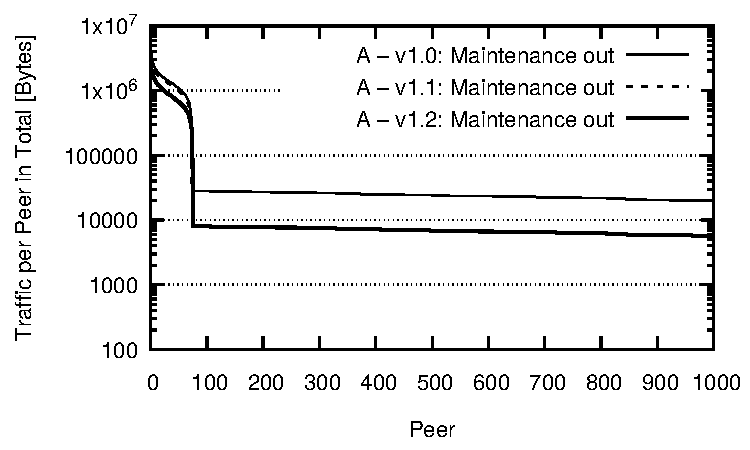
\includegraphics[width=0.98\linewidth]{graphics/fig/Maintenance_Traffic_Peers_A_out}
  }
  \\[-1ex]
  \subfigure[A: 1.0 $\rightarrow$ 1.1 $\rightarrow$ 1.2 -- Incoming traffic, 3 features, no churn\label{fig:traffic_peers_A_in}] {\centering
  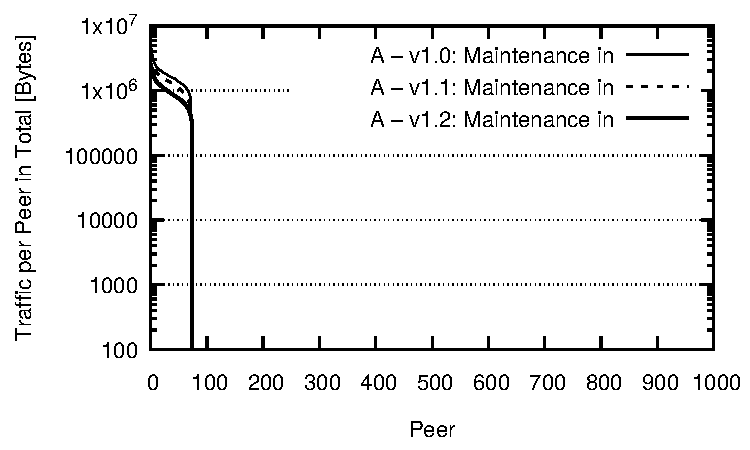
\includegraphics[width=0.98\linewidth]{graphics/fig/Maintenance_Traffic_Peers_A_in}
  }
  \\[-1ex]
  \subfigure[C: 1.0 $\rightarrow$ 1.1 $\rightarrow$ 1.2 -- Outgoing traffic, 5 features, churn\label{fig:traffic_peers_C_out}] {\centering
  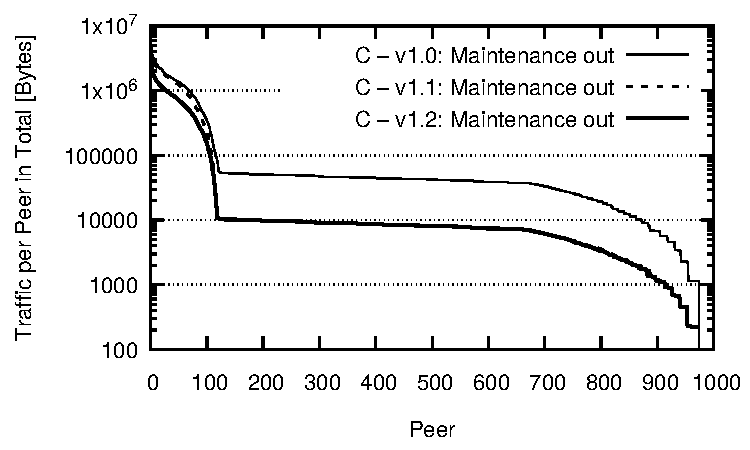
\includegraphics[width=0.98\linewidth]{graphics/fig/Maintenance_Traffic_Peers_C_out}
  }
  \\[-1ex]
  \subfigure[C: 1.0 $\rightarrow$ 1.1 $\rightarrow$ 1.2 -- Incoming traffic, 5 features, churn\label{fig:traffic_peers_C_in}] {\centering
  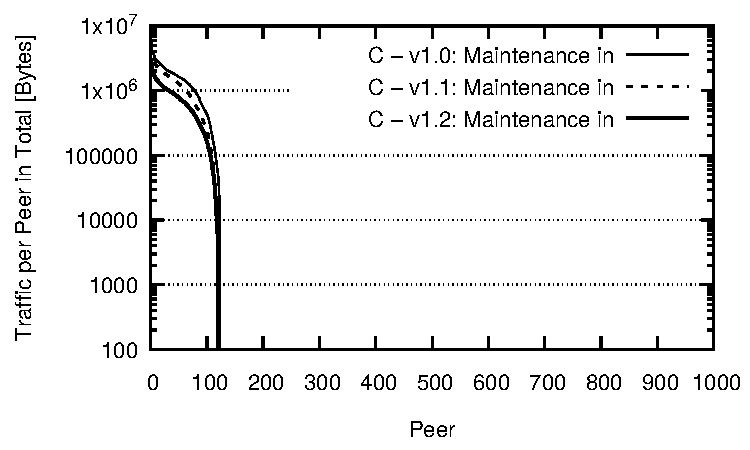
\includegraphics[width=0.98\linewidth]{graphics/fig/Maintenance_Traffic_Peers_C_in}
  }
  \\[-1ex]

  \caption{Protocol revisions v1.1 + v1.2 -- maintenance traffic by peers}
  \label{fig:traffic_peers}
\end{figure}

\begin{figure}[htbp]
  \centering

  \subfigure[A: 1.0 $\rightarrow$ 1.1 $\rightarrow$ 1.2 -- 3 features, no churn\label{fig:traffic_time_A}] {\centering
  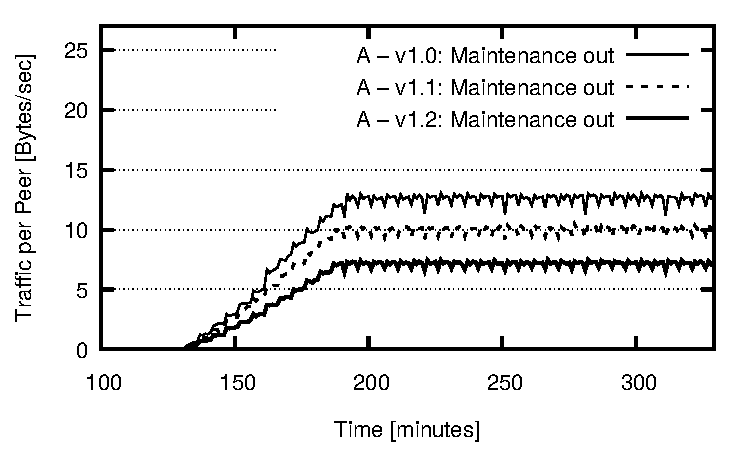
\includegraphics[width=0.98\linewidth]{graphics/fig/Maintenance_Traffic_Time_A_11+12}
  }
  \\[-1ex]
  \subfigure[C: 1.0 $\rightarrow$ 1.1 $\rightarrow$ 1.2 -- 5 features, churn\label{fig:traffic_time_C}] {\centering
  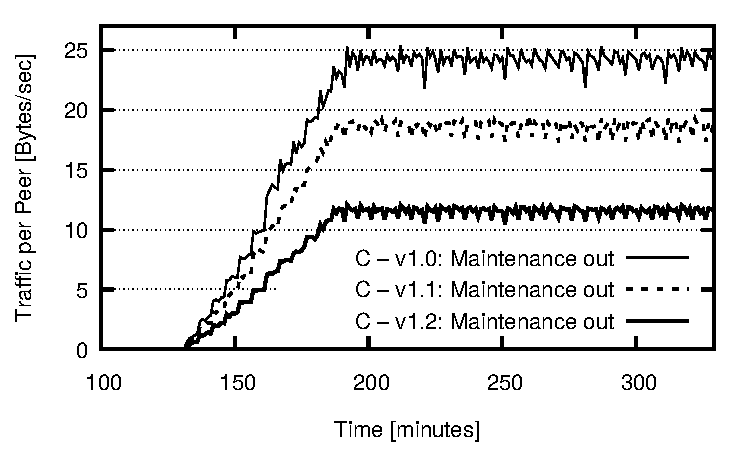
\includegraphics[width=0.98\linewidth]{graphics/fig/Maintenance_Traffic_Time_C_11+12}
  }
  \\[-1ex]

  \caption{Protocol revisions v1.1 + v1.2 -- maintenance traffic by time}
  \label{fig:traffic_time}
\end{figure}


For evaluating the protocol revisions our metrics are 
\begin{inparaenum}[i)]
  \item maintenance traffic costs to PacketSkip,
  \item maintenance traffic costs between PacketSkip nodes,
  \item storage costs,
  \item impact on search duration and search hops and
  \item global PacketSkip traffic costs.
\end{inparaenum}
For the evaluation of the host cache we examine the following metrics:
\begin{inparaenum}[i)]
  \item search and update duration,
  \item performance under churn and
  \item effects on global overlay traffic costs.
\end{inparaenum}

PacketSkip has been implemented in the PeerfactSim.KOM~\cite{peerfactsim} p2p simulator. All changes are evaluated inside this simulation framework. For consistency we rely on the basic scenarios already introduced in \cite{packetskip10}. See Table~\ref{tab:eval_scenario} for details. Scenario A runs without churn, while scenario B and C uses churn with a Kad-distribution. Scenarios A and B use 3 capacity features, with scenario C we used 5 features. For each basic scenario a $k=8$ search and a full search have performed.

For comparison of the different revisions each basic scenario has been simulated with the following parameters:

\begin{enumerate}
  \item[1.0)] protocol v1.0 (as reference)
  \item[1.0c)] protocol v1.0 + cache
  \item[1.1)] protocol v1.1 (adding additional features on the receiving node, not using the suffix model)
  \item[1.2)] full protocol v1.2 (restrict additional features to lexicographical suffixes, includes v1.1)
  \item[1.2c)] full protocol v1.2 (includes v1.1) + cache
\end{enumerate}

We will not expand on all possible combinations A:1.0 to C:1.2c, but only on those with meaningful relevance. Scenario C for example is mostly of interest for the protocol changes and not for the host cache. All scenarios have been simulated with 10 different seeds. For a full overview on all parameters, please refer to Table~\ref{tab:eval_param}. We have used an ideal net layer with a small, constant latency and also a fixed timeout for cache misses.







\subsection{Protocol revision v1.1 and v1.2 -- maintenance traffic costs}
\label{subsec:11}

At first, we evaluate the effects of the protocol enhancement on messages sent to and between PacketSkip nodes.
Figure~\ref{fig:traffic_peers} illustrates the incoming and outgoing maintenance traffic of the service, which includes messages for graph maintenance and especially for index updates, sorted by peers (highest load to the left). The bump on the left side is caused by peers which maintain a PacketSkip node. Peers on the right side are just pushing their update messages. 
For the latter the reduction in output message traffic from v1.0 to v1.1 is apparent.
This was to be expected, since v1.1 eliminates redundancies in update messages sent to PacketSkip.
As v1.2 incorporates v1.1, the effects are identical here (Fig.~\ref{fig:traffic_peers_A_out}: curves of v1.1 and v1.2 are overlapping).
Peers with PacketSkip nodes see positive effects on the incoming side (Fig.~\ref{fig:traffic_peers_A_in}). 

V1.2 on the other hand also reduces the traffic costs inside PacketSkip, demonstrated by less deflection on the left side. This is due to the reduced sizes of the additional feature sets. The effects become more obvious with an increased number of features (scenario C, Fig.~\ref{fig:traffic_peers_C_out}, \ref{fig:traffic_peers_C_in}).
% With 5 capacity features, the number of PacketSkip nodes increases, broadening the bump on the left to some extent. The drop-off to the right is simply caused by churn.

If we average the maintenance traffic over all peers, we notice the effects on the overall maintenance costs of PacketSkip, i.e. messages to the service and between the nodes. There is a noticeable reduction from v1.0 (12.6 Bytes/sec) to v1.1 (10.0 Bytes/sec) to v1.2 (7.2 Bytes/sec) (3 features -- Fig.~\ref{fig:traffic_time_A}), respectively from 24.2 to 18.6 to 11.5 Bytes/sec (5 features -- Fig.~\ref{fig:traffic_time_C})








\subsection{Protocol revision v1.2 -- storage costs}
\label{subsec:dht}

The second protocol revision stores only lexicographical suffixes as additional features. Evaluation proofs that halving the additional features leads to a significant drop of storage requirements, especially with increasing dimensionality (see Fig.~\ref{fig:dht} -- note the log scale of the abscissa). The steps represent peers with one or more PacketSkip nodes. Storage requirements grow almost linearly with the number of nodes a peer maintains. Averaging on all peers, we have measured a reduction from 0.38 to 0.23 KBytes (3 features) and 0.60 to 0.33 KBytes (5 features), which is consistent with the prediction.

  \begin{figure}[htbp]
    \centering
    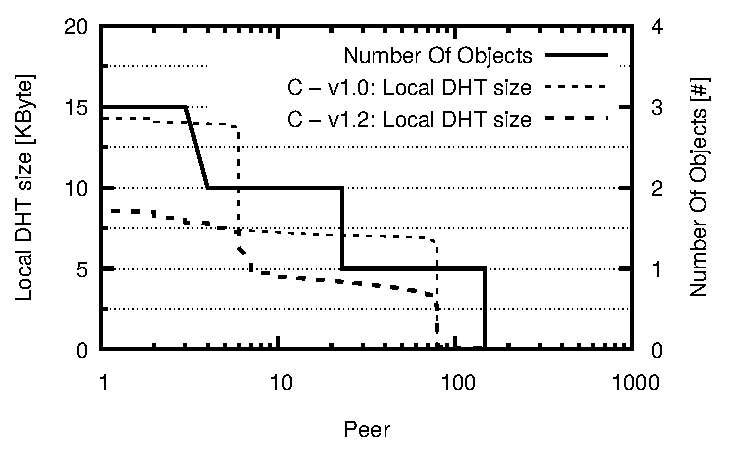
\includegraphics[width=0.98\linewidth]{graphics/fig/DHTSize_PeersSort_C}
    \\[-1ex]
    \caption{C: 1.0 $\rightarrow$ 1.2 -- Storage requirements per peer, 5 capacity features}
    \label{fig:dht}
  \end{figure}



\subsection{Protocol revision v1.2 -- search performance}
\label{subsec:search}

\begin{figure}[htbp]
  \centering

  \subfigure[A: v1.0 -- Search durations, full-search\label{fig:search_duration_nochurn_10c_fs}] {\centering
  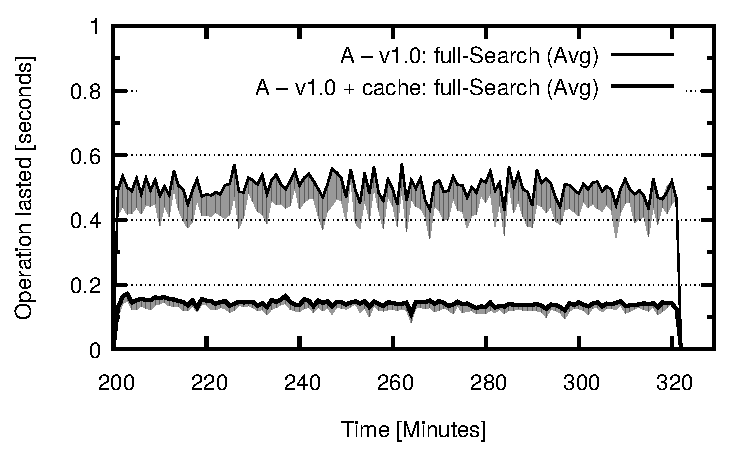
\includegraphics[width=0.98\linewidth]{graphics/fig/Search_Duration_A_10c_fs}
  }
  \\[-1ex]
  \subfigure[A: v1.2 -- Search durations, full-search\label{fig:search_duration_nochurn_12c_fs}] {\centering
  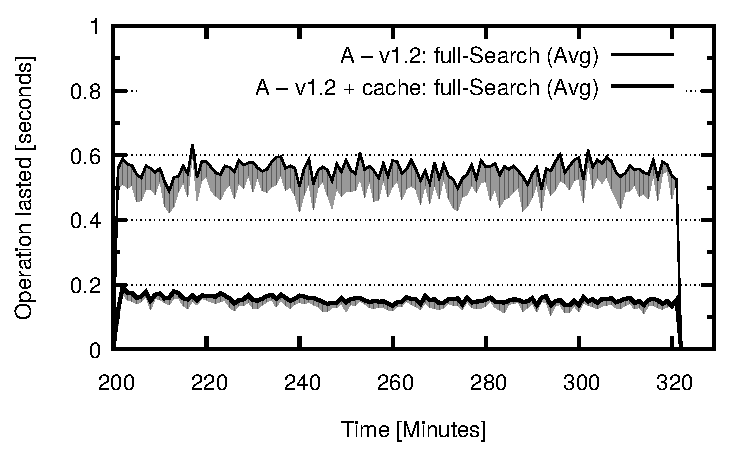
\includegraphics[width=0.98\linewidth]{graphics/fig/Search_Duration_A_12c_fs}
  }
  \\[-1ex]
  \subfigure[A: v1.0 -- Search durations, k-search\label{fig:search_duration_nochurn_10c_ks}] {\centering
  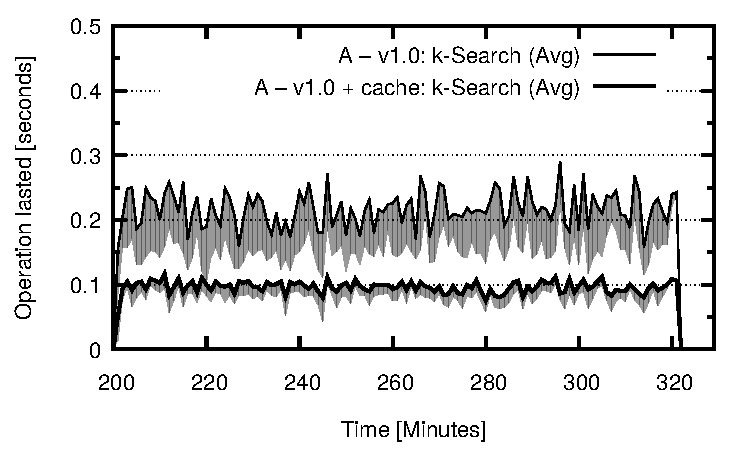
\includegraphics[width=0.98\linewidth]{graphics/fig/Search_Duration_A_10c_ks}
  }
  \\[-1ex]
  \subfigure[A: v1.2 -- Search durations, k-search\label{fig:search_duration_nochurn_12c_ks}] {\centering
  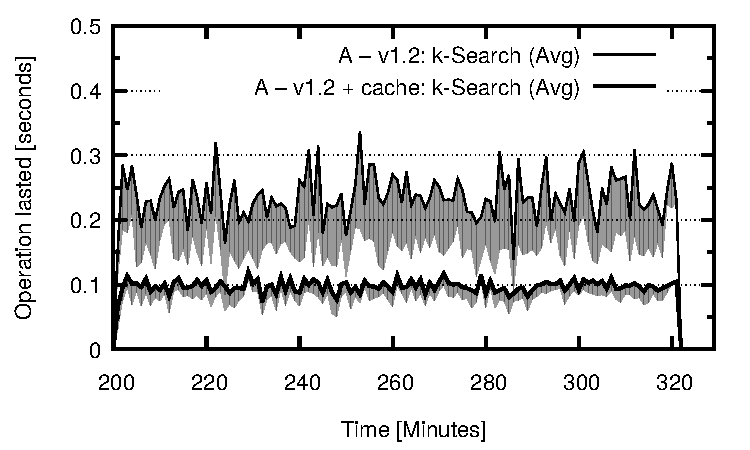
\includegraphics[width=0.98\linewidth]{graphics/fig/Search_Duration_A_12c_ks}
  }
  \\[-1ex]

  \caption{Effetcs of cache and protocol v1.2 on search durations, no churn}
  \label{fig:search_durations_nochurn}
\end{figure}

On the downside, the search duration is slightly affected in v1.2, especially for full searches (compare full-search: Fig.~\ref{fig:search_duration_nochurn_10c_fs} to \ref{fig:search_duration_nochurn_12c_fs}, and k-search: Fig.~\ref{fig:search_duration_nochurn_10c_ks} to \ref{fig:search_duration_nochurn_12c_ks}).
Table~\ref{tab:durations} lists the average search durations for several scenarios.

There is an even more pronounced increase in contacted nodes for a search (search hops), especially for full searches, which is roughly doubling in number (Fig.~\ref{fig:search_hops}).
This is due to the fact that nodes are not allowed to focus their search on the feature with the smallest search range. It is however noteworthy, that our simulations randomized only the lower bound for a search interval. The upper bound is always unlimited. In other words, seekers always search for all occurrences greater or equal a random value. Under this condition a smaller search range is always a best choice. So, we have basically chosen a worst case scenario for the evaluation of the v1.2 protocol revision.

Having said this, the full bandwidth costs for PacketSkip messages (maintenance and search combined) compared to the top 4 overlay message types are clearly enhanced with protocol v1.2 (compare Fig.~\ref{fig:net_C_10} to \ref{fig:net_C_12}).

\begin{figure}[t!]
  \centering
  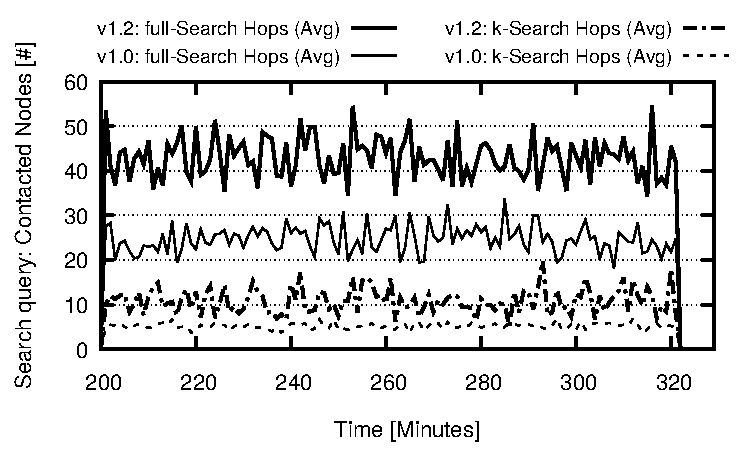
\includegraphics[width=0.98\linewidth]{graphics/fig/Search_Hops}
  \\[-1ex]
  \caption{Effects of protocol revision v1.2 on search hops (full and k-search)}
  \label{fig:search_hops}
\end{figure}


\begin{table}[hb]
\centering
\caption{Average search and update duration times [seconds]}
\label{tab:durations}
\begin{tabular}{|c|c|c|c|c|c|}
\hline
\multirow{2}{*}{\textbf{Scenario}} & \multirow{2}{*}{\textbf{Action}} & \multicolumn{2}{c|}{\textbf{no cache}} & \multicolumn{2}{c|}{\textbf{cache}} \\ \cline{3-6} 
                                   &                                  & \textbf{v1.0}      & \textbf{v1.2}     & \textbf{v1.0}    & \textbf{v1.2}    \\ \hline
                                                                                                                                                        \hline
\multirow{3}{*}{A}                 & Full-Search                      & 0.47               & 0.52              & 0.13             & 0.14             \\ \cline{2-6} 
                                   & k-Search                         & 0.20               & 0.22              & 0.09             & 0.09             \\ \cline{2-6} 
                                   & Update                           & 0.41               & 0.42              & 0.13             & 0.12             \\ \hline
\multirow{3}{*}{B}                 & Full-Search                      & 2.72               & 3.75              & 1.50             & 2.07             \\ \cline{2-6} 
                                   & k-Search                         & 1.11               & 1.18              & 0.64             & 0.84             \\ \cline{2-6} 
                                   & Update                           & 2.06               & 2.05              & 1.31             & 1.19             \\ \hline
\end{tabular}
\end{table}




\subsection{Host cache}
\label{subsec:10c}

We now examine the results of the new host caching component.
As predicted, search and update duration times were considerably reduced in scenario A.
Durations are reduced by a factor of 3.1 on average (Fig.~\ref{fig:search_durations_nochurn}, \ref{fig:update_duration_nochurn_10c}, also table ~\ref{tab:durations}).

A cache may lead to cache misses under churn, so we had to verify its benefits in a more dynamic scenario (B). 
Figures~\ref{fig:search_duration_churn_10_ks} and \ref{fig:search_duration_churn_10c_ks} in comparison demonstrate that our caching mechanism lead to fewer spikes under churn and actually helped to reduce the negative effects of churn on the search duration. 
The update duration is also improved under churn (Fig.~\ref{fig:update_duration_churn_10c}). We measure a reduction of factor 1.7 for searches and updates on average in scenario B (Table~\ref{tab:durations}).


\begin{figure}[htbp]
  \centering

  \subfigure[B: 1.0 -- Search durations without cache under churn\label{fig:search_duration_churn_10_ks}] {\centering
  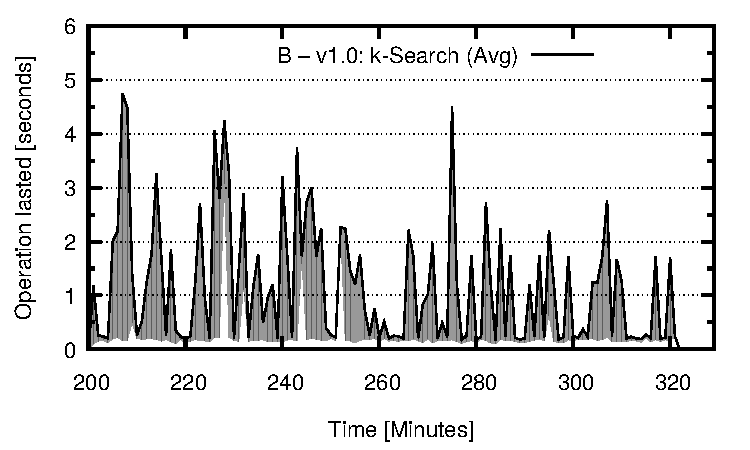
\includegraphics[width=0.98\linewidth]{graphics/fig/Search_Duration_B_10}
  }
  \\[-1ex]
  \subfigure[B: 1.0c -- Search durations with cache under churn \label{fig:search_duration_churn_10c_ks}] {\centering
  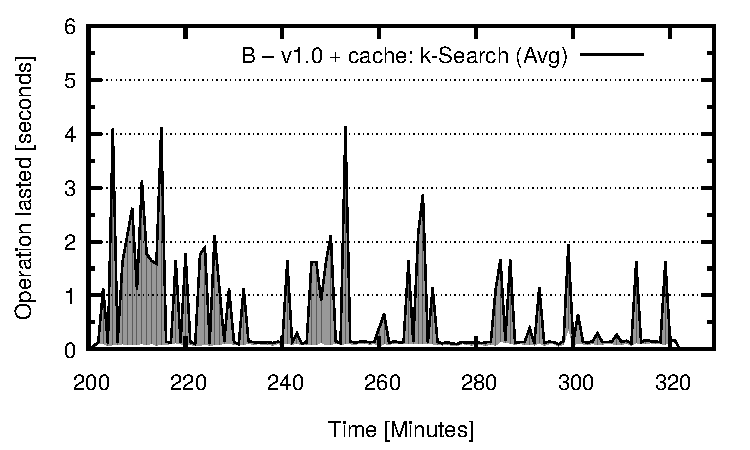
\includegraphics[width=0.98\linewidth]{graphics/fig/Search_Duration_B_10c}
  }
  \\[-1ex]
  \subfigure[A: 1.0 $\rightarrow$ 1.0c -- Update durations, no churn\label{fig:update_duration_nochurn_10c}] {\centering
  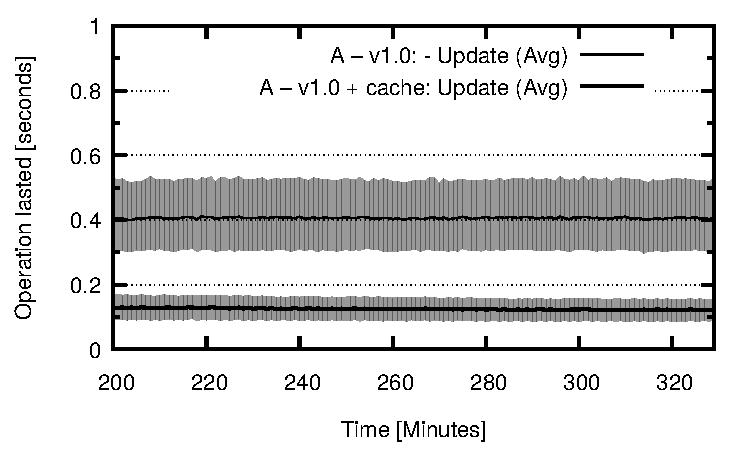
\includegraphics[width=0.98\linewidth]{graphics/fig/Update_Duration_A_10+10c}
  }
  \\[-1ex]
  \subfigure[B: 1.0 $\rightarrow$ 1.0c -- Update durations under churn\label{fig:update_duration_churn_10c}] {\centering
  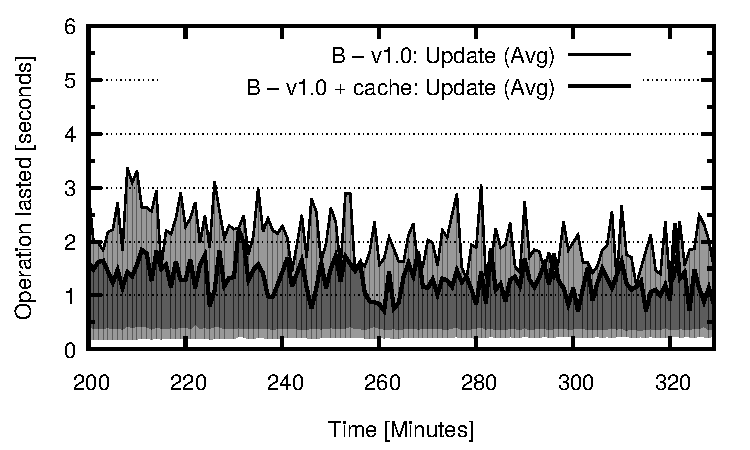
\includegraphics[width=0.98\linewidth]{graphics/fig/Update_Duration_B_10+10c}
  }
  \\[-1ex]

  \caption{V1.0 with cache: influence on search and update durations}
  \label{fig:durations_cache}
\end{figure}






\subsection{Joint enhancements}
\label{subsec:12c}

By avoiding unnecessary lookups we can notably reduce the overlay and lookup traffic caused by PacketSkip. Figure~\ref{fig:net_C_12c} demonstrates the positive effects of all proposed protocol changes in cooperation with the host cache. The entire overlay communication costs are reduced, not only with respect to PacketSkip messages, but especially regarding lookup costs.

As a final note: our evaluation recorded no impact to the accuracy (precision, false positives) of PacketSkip's search results by introducing protocol revisions and host cache.

\begin{figure}[htbp]
  \centering

  \subfigure[C: protocol v1.0\label{fig:net_C_10}] {\centering
  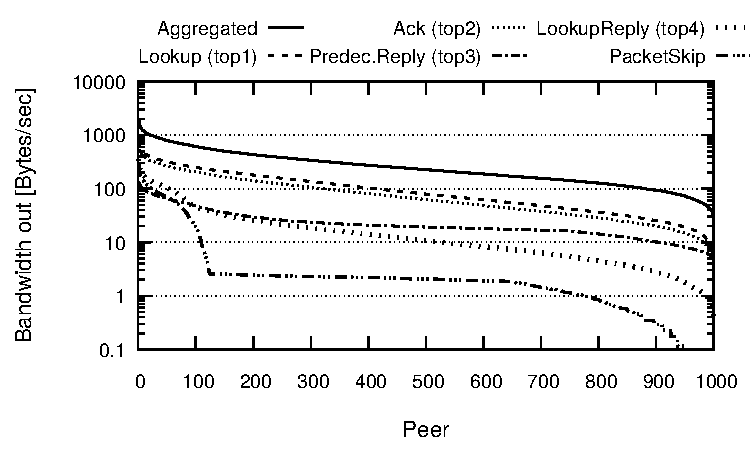
\includegraphics[width=0.98\linewidth]{graphics/fig/Top5_Traffic_Peers_C_10}
  }
  \\[-1ex]

  \subfigure[C: protocol v1.2\label{fig:net_C_12}] {\centering
  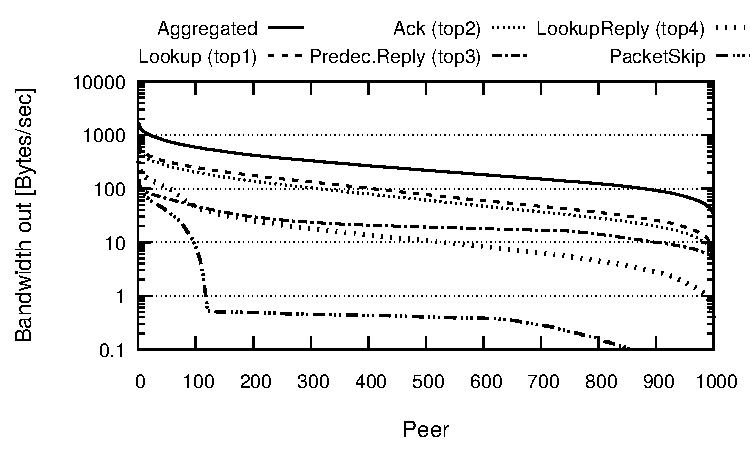
\includegraphics[width=0.98\linewidth]{graphics/fig/Top5_Traffic_Peers_C_12}
  }
  \\[-1ex]
  \subfigure[C: protocol v1.2 + cache\label{fig:net_C_12c}] {\centering
  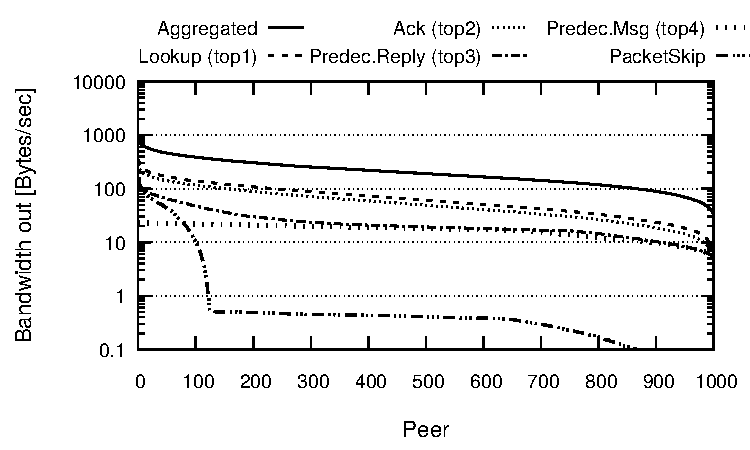
\includegraphics[width=0.98\linewidth]{graphics/fig/Top5_Traffic_Peers_C_12c}
  }
  \\[-1ex]

  \caption{Global overlay traffic: top 4 message types vs PacketSkip}
  \label{fig:net}
\end{figure}

